% Overleaf: upload this file together with stage2_ri_vs_causal_effect.png
% and compile with pdfLaTeX.
\documentclass[11pt,a4paper]{article}
\usepackage[margin=2.2cm]{geometry}
\usepackage[T1]{fontenc}
\usepackage[utf8]{inputenc}
\usepackage{lmodern,microtype}
\usepackage{amsmath,booktabs,graphicx}
\usepackage{xcolor}
\usepackage[colorlinks=true,urlcolor=blue!60!black]{hyperref}
\setlength{\parindent}{0pt}
\setlength{\parskip}{5pt}
\setlength{\emergencystretch}{2em}
\renewcommand{\arraystretch}{1.15}

\title{Stage 2: Results and Analysis\\\large Single-hop Causal Head Map in OLMo-2-7B}
\author{Daniella Simonovsky and Max Golubkov}
\date{September 2026}

\begin{document}
\maketitle

\section{Run and validation}
Run \texttt{stage2\_v1} completed successfully as Slurm job 888691 in 1h14m42s
with exit code 0. Three persistent replicas used six GPUs in total, with two
GPUs per replica. The run used the base \texttt{allenai/OLMo-2-1124-7B} model,
revision \texttt{7df9a82518afdecae4e8c026b27adccc8c1f0032}, and the same
data, behavioral baseline, discovery split, and Stage-1 artifacts as the
observational scan.

All mandatory gates passed independently on all three replicas. The behavioral
runner drift, self-patch drift, self-attribution effect, and corrupted-input
embedding endpoint drift were zero on the checked examples. The gate also
covered shared-answer-prefix cases and exact versus gradient previews. These
checks establish consistency of this implementation on the tested inputs; they
do not establish scientific usefulness of any head.

The output is complete: all 178 clean/corrupted discovery pairs have finite
screen and extension files; 40 pairs have exact effects for all 1,024 heads;
and all 178 pairs have exact effects for the 92-head extension set. The raw
arrays reproduce \texttt{head\_effects.csv}. Model, data, baseline, Stage-1,
and code hashes match the saved manifest.

\section{Intervention and outcome measure}
For each family and fact order, let $x_c$ be the clean prompt and $x_r$ its
token-aligned corrupted twin. The corruption swaps the two answer-side names in
the facts, so that the clean distractor becomes the corrupted answer. If the two
answer strings share a token prefix $c$, the metric is evaluated at their first
divergent token:
\begin{equation}
M(x)=\operatorname{logit}(y_c\mid x,c)-
     \operatorname{logit}(y_r\mid x,c).
\end{equation}
The sign is fixed to the clean answer on both inputs. Thus, $M(x_c)>0$ and
$M(x_r)<0$ indicate that the model tracks the changed fact. Four of the 178
pairs had a non-empty shared answer prefix.

For head $h$, exact patching replaces its slice of the input to the attention
output projection with the activation from the corrupted run at every original
prompt position. Shared answer-prefix positions are recomputed. Define
\begin{equation}
\Delta_h=M(x_c; a_h\leftarrow a_h^{r})-M(x_c),
\qquad I_h=-\Delta_h.
\end{equation}
We report $I_h$ as \emph{causal importance}: a positive value means that the
patch moves the metric toward the corrupted answer. It is measured in logits.
It is not an accuracy difference, a sequence-likelihood difference, or an
additive decomposition of the clean--corrupted gap.

Across the 89 discovery families, averaging the two orders within each family,
the mean clean metric was 5.680 (95\% family-bootstrap interval
$[5.338,6.030]$), while the corrupted metric with the clean sign fixed was
$-5.491$ ($[-5.850,-5.141]$). The mean gap was 11.170
($[10.632,11.725]$). Every clean pair had positive $M$ and every corrupted pair
had negative $M$. The intervention contrast is therefore behaviorally strong
and sign-consistent.

Intervals in this report are descriptive percentile bootstrap intervals from
20,000 resamples of whole families (seed 20260915), after averaging the two
orders. They were computed after observing the Stage-2 results and are not
additional pre-registered hypothesis tests.

\section{The first-order screen is well calibrated}
The first-order estimate contracts the clean-to-corrupted head-output change at
all original prompt positions with the gradient of $M$ at the clean run. On the
40-pair exact subset, using the same pairs for both methods, its signed
head-ranking Spearman correlation with exact patching was 0.945. The correlation
of absolute mean effects was 0.921, and the pair-by-head correlation was 0.903.
This passed the pre-registered threshold of 0.7, so the five-step
input-embedding IG fallback was correctly not used.

Two further comparisons separate approximation error from family-sampling
variation. Comparing the attribution mean over all 178 pairs with the exact mean
over only the 40-pair subset gives a lower correlation of 0.698. In contrast,
among the 92 extension heads, attribution and exact patching evaluated on the
same 178 pairs correlate at 0.990. The lower cross-sample value is therefore not
evidence that the screen failed; it mixes approximation error with a change in
the evaluated families.

\section{Causal map}
Table~\ref{tab:top} reports the strongest heads in the all-family exact
extension. The extension set was selected on the discovery data using RI,
attribution, fixed Stage-1 examples, and random controls. The intervals therefore
describe effect stability within this run; they are not selection-adjusted
confidence statements.

\begin{table}[ht]
\centering
\small
\begin{tabular}{lrrrr}
\toprule
Head & RI & Attribution & Exact $I_h$ & Gap fraction \\
\midrule
L17H1  & .0094 & 3.362 & 5.701 $[5.294,6.112]$ & .510 \\
L18H19 & .0182 & 2.785 & 3.072 $[2.867,3.276]$ & .275 \\
L27H6  & .0000 & 2.640 & 3.071 $[2.749,3.390]$ & .275 \\
L18H18 & .0151 & 2.226 & 2.704 $[2.503,2.907]$ & .242 \\
L21H18 & .0096 & 1.480 & 1.704 $[1.588,1.822]$ & .153 \\
L25H17 & .0116 & 1.183 & 1.267 $[1.190,1.342]$ & .113 \\
L22H5  & .0155 & .950 & .983 $[.904,1.063]$ & .088 \\
L16H21 & .0240 & .695 & .925 $[.808,1.049]$ & .083 \\
L16H1  & .0137 & .812 & .868 $[.766,.972]$ & .078 \\
L21H6  & .0067 & .662 & .702 $[.636,.770]$ & .063 \\
\bottomrule
\end{tabular}
\caption{Strongest exact effects among the 92 extension heads. Gap fraction is
$I_h$ divided by the mean 11.170-logit clean--corrupted gap. It must not be
summed across heads because single-head patching effects can interact.}
\label{tab:top}
\end{table}

L17H1 is unusually strong: replacing this one head moves the metric by 5.701
logits on average, approximately 51\% of the full clean--corrupted gap. Its
effect had the expected sign in every family. L18H19, L27H6, and L18H18 each
account individually for approximately one quarter of the gap, again with the
expected sign in every family. These magnitudes establish intervention
sensitivity, not four independent shares of a decomposition.

The all-head exact map used a randomly chosen set of 20 whole families, both
orders. Its top four heads were the same four shown above, and their effect
magnitudes closely reproduced the 89-family extension: L17H1, L27H6, L18H19,
and L18H18 had subset effects 5.742, 3.222, 3.080, and 2.768. The large effects
are therefore not artifacts of reporting only the all-family extension.

Across all 1,024 heads, the order-0 versus order-1 exact ranking correlation was
0.461. This value is dominated by the many heads whose effects are near zero.
Within the selected 92 heads the correlation was 0.734, and among the overall
top 25 it was 0.656; 17 heads appeared in both order-specific top-25 lists. All
ten heads in Table~\ref{tab:top} had positive mean importance in both orders.
Thus the main effects are not confined to one layout, while weaker-head ordering
is less stable.

\begin{figure}[ht]
\centering
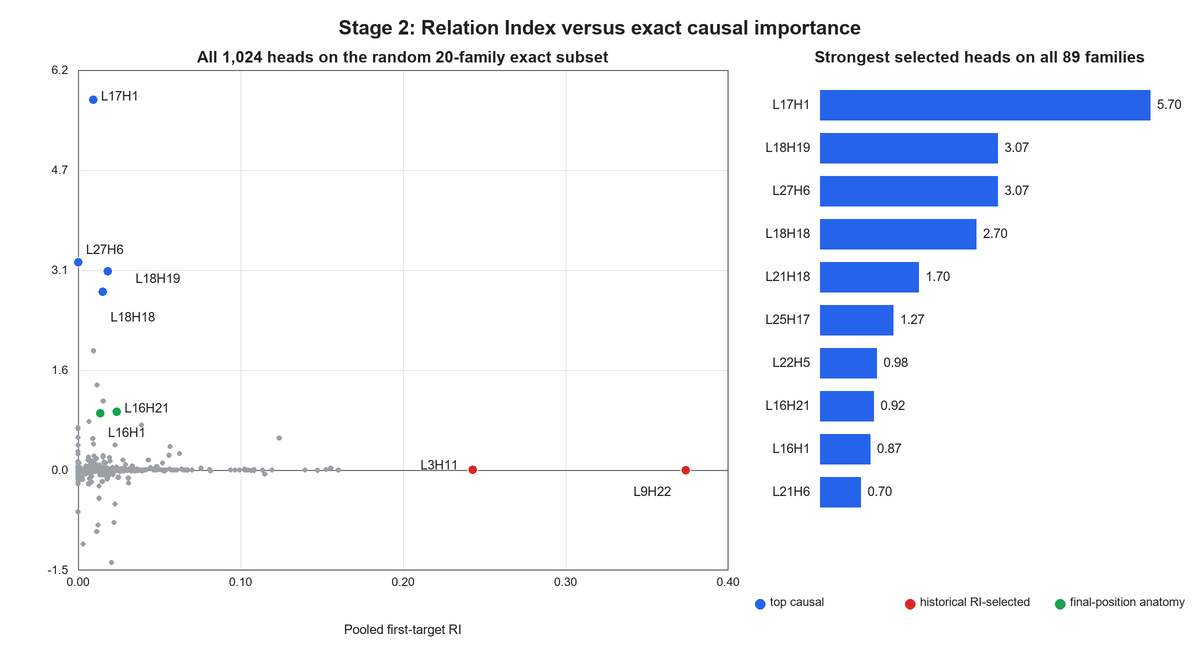
\includegraphics[width=\textwidth]{stage2_ri_vs_causal_effect.png}
\caption{Stage-2 causal map. Left: pooled first-target RI versus exact causal
importance for all 1,024 heads on the random 20-family subset. Right: strongest
heads among the 92-head exact extension on all 89 discovery families. The
historical RI-selected heads lie near zero causal importance, while the largest
causal effects have low RI.}
\label{fig:map}
\end{figure}

\section{RI has weak correspondence with causal importance}
The Spearman correlation between pooled first-target RI and exact importance
over all heads was 0.135 on the random exact subset. A family bootstrap gave a
descriptive stability interval of $[0.063,0.168]$. The last-target sensitivity
score performed similarly ($\rho=0.132$). These small positive associations do
not support RI as a useful causal ranking for this task.

Only one of the exact top-25 heads appeared in the supported RI-first top 25,
and only one appeared in the RI-last top 25. By comparison, 17 of the exact
top-25 appeared in the attribution top 25. The overlap result agrees with the
rank correlations: the gradient screen tracks exact effects, whereas the RI
ranking mostly selects different heads.

The historical pooled rule had selected L3H11 and L9H22. On all 89 families,
their exact importance was $-0.0022$ ($[-0.0067,0.0024]$) and $-0.0020$
($[-0.0065,0.0027]$), with the expected sign in only 47\% and 42\% of families.
Their median importance was $-0.0021$, compared with $0.0002$ for the 25 random
extension controls. These heads therefore have no detectable effect under this
single-head, all-prompt-position patching experiment.

This result sharpens the Stage-1 event analysis. L3H11's RI events were all
previous-token attention from the same period/newline token, and L9H22's events
were all self-attention. More than 99\% of their summed first-target scores came
from demonstrations. Stage 2 now shows that the large observational scores do
not translate into movement of the answer metric when their contextual head
activations are transplanted.

\section{Pre-registered audit verdicts}
The earlier methodology defined three non-exclusive verdicts. The available
evidence supports the following reading.

\textbf{Incomplete: supported.} The lenient 99th percentile of the historical
random-token control means was 0.1374. Of the 102 heads in the top decile of
positive exact effect, 101 fell below this threshold and 24 had RI exactly zero.
Most decisively, L27H6 ranked second in exact importance but had RI zero. Thus a
large causal effect can lie below even the lenient RI threshold; this conclusion
does not depend on choosing a stricter cutoff after observing Stage 2.

\textbf{Misleading: descriptively supported.} The pre-registered criterion asked
whether the median causal effect of RI-passing heads exceeded that of random
heads. It did not: the two historical RI-passing heads had median importance
$-0.0021$, versus $0.0002$ for the random controls. The historical RI threshold
itself was a descriptive cross-head percentile rather than a calibrated
per-head significance test, so this verdict should be reported with that
qualification.

\textbf{Sound: not supported.} The methodology described soundness as
systematically larger effects for RI-passing heads than for layer-matched
non-passing heads, but did not fully operationalize the comparison. Only two
heads passed the historical rule, one of which ranked high within its early
layer on the 20-family subset but had a tiny effect that vanished on the full
89-family extension. The present data therefore do not support soundness, but
we do not turn the underspecified criterion into a new post-hoc significance
test.

These verdicts concern the implemented RI adaptation and causal experiment on
this dataset. They are not a universal rejection of semantic induction heads or
of attention-based diagnostics.

\section{Two distinct ways RI misses important heads}
The combination of Stage-1 events and Stage-2 effects suggests at least two
failure modes.

\textbf{QK-selection miss.} L17H1 had only two scored Stage-1 QK passes across
the full scan, yet it was the strongest causal head by a large margin. Its
mechanism therefore rarely satisfies the specific condition that the annotated
source token be the unique dominant attention target by a factor greater than
2.2. It may distribute attention, retrieve through a different position, or
operate on information already moved by upstream components.

\textbf{Raw-embedding OV miss.} L27H6 had 85 scored QK passes but pooled RI zero,
despite an exact effect of 3.071 logits. This separates attention eligibility
from the embedding-level OV score. A head can be causally important even when
$e_jW_V^hW_O^hW_U$ does not promote the annotated target token. Its actual
contextual input may carry information absent from the raw token embedding, or
its downstream effect may be indirect rather than a direct target-token write.

L16H1 and L16H21 provide a third informative pattern. Stage 1 found 223 and 230
dominant-attention events, respectively, from the final prompt token to
test-fact sources across 76 and 79 families. Stage 2 found exact effects of
0.868 and 0.925 logits. This agreement makes them promising query-position
retrieval candidates. However, their low pooled RI shows that the full RI
definition still under-ranks them, plausibly because its raw-embedding OV term
does not measure their contextual output.

L16H4, which had the smallest raw matched-target calibration $p$ value in
Stage 1 and 63 final-position source-attention events, had a positive but much
smaller exact effect: 0.0257 logits ($[0.0190,0.0328]$), approximately 0.2\% of
the clean--corrupted gap. Dominant source attention and a weak target preference
can therefore coexist with only a small causal effect on the answer contrast.

\section{Interpretation and next mechanistic questions}
Stage 2 establishes a reliable causal screen under a precisely specified
intervention. It provides strong evidence that the implemented RI definition is
not a complete causal account of the model's single-hop relational behavior.
It also identifies a compact set of robust intervention-sensitive heads,
concentrated mainly in layers 16--27, for the next stage.

The result does \emph{not} yet identify a circuit. Because each patch replaced a
head at all original prompt positions, it does not localize the effect to the
question, relevant fact, or answer-prediction position. A large effect may
reflect semantic relation processing, entity binding, name copying, or another
feature that differs between the token-aligned twins. Single-head effects also
do not establish necessity under redundancy, edges between heads, or additive
composition.

Stage 3 should therefore begin with L17H1, L18H19, L27H6, L18H18, L16H1, and
L16H21, while retaining the original RI heads and random controls. The first
questions are:
\begin{enumerate}
\item At which prompt positions does each exact effect arise?
\item Where does each head attend on clean and corrupted twins, and does the
attention track the query-relevant fact rather than a fixed location?
\item What does the head's \emph{actual contextual output}, rather than its raw
embedding OV projection, write into the residual stream?
\item Which upstream components supply its queries, keys, and values, and which
downstream components consume its output?
\item Do pairwise and group interventions reveal redundancy or nonlinear
interactions that single-head patches cannot detect?
\end{enumerate}
Only after these position- and edge-level tests should the components be called
a semantic circuit or evaluated for minimal-circuit faithfulness on the held-out
validation families.

\section{Conclusion}
The causal map changes the Stage-1 picture. The two heads selected by pooled RI
have essentially zero exact effect, while several low-RI heads have large,
stable, and correctly signed effects. The first-order screen is strongly
validated against exact patching, so this contrast is not explained by a failed
approximation. Within the implemented task and patching scope, RI is incomplete
and descriptively misleading as a causal selection rule. The main positive
result is not merely that RI fails: Stage 2 identifies a reproducible set of
mid-to-late-layer heads whose mechanisms can now be tested at position and edge
resolution.

\end{document}
